%
%   N A M B A   N A M B A   N A M B A
%    N A M B A   N A M B A   N A M B A
%     N A M B A   N A M B A   N A M B A
%

\documentclass[10pt,b5paper,papersize,dvipdfmx]{jsbook}

\usepackage{vuccaken}
\usepackage{vuccaken2019}

% スタイルファイルの読み込みや自作マクロは、
% 最終的には vuccaken2019.sty の中に書いてください。
% とりあえずはここに書いてもらって構いません。


\begin{document} % 以下本文

\mokuji{2} % 目次出力

% - - - - - - - - - - - - - - - - - - - - - - - - %
\kaishititle%
  {流体中の物体に働く揚力}% title
  {物理科学科1回生}% 所属
  {\vname{難波}{潤}}% name
% - - - - - - - - - - - - - - - - - - - - - - - - %

%
\section*{はじめに}
流体は我々の身の周りに存在していながら、我々の目にはみえない不思議な運動をする。
ここでは様々な流体の運動のうち、揚力に着目し簡潔に解説したいと思う。

\section{そもそも流体とは?}
流体は、簡単に言えば自由に変形できる物質である。液体と気体がそれにあたり、特定の形を持たず容易に変形し、接する固体の形状によって運動が支配される。
流体の特徴として粘性と呼ばれるものがある。これは流体中を運動する物体に対して、流体が変形を妨げようとして抵抗を示す性質である。例として、管の中に流体を通すと流体が管の壁と接する部分は管の中心部に比べて速度が遅くなる。これは粘性の働きによるものである。実在する流体はごく一部の例外を除きこの粘性を考慮する必要がある。
\par
流体は圧力によって圧縮され体積を変化させる性質(圧縮性)をもつが、圧縮性及び粘性を無視した流体を理想流体という。仮に理想流体を管に流した場合、管の壁付近と中心部での速度は等しくなる。ただし、理想流体は粘性がないためエネルギー損失や抵抗力が存在せず、実在する気体と矛盾する。
一方、実在流体を壁付近で粘性の影響を大きく受けて速度が遅い領域(境界層)と壁から離れた境界層より外側の領域(主流)に分けると、主流領域では粘性の影響が小さく、理想流体とみなすことができる。

\subsection{揚力}
揚力と聞くと物体を下から上に持ち上げる力を連想するかもしれないが、実は少し違う。揚力とは、物体に働く力のうち、流れの方向に垂直な成分のことである。(重力は例外)つまり流れの方向及び物体の運動の方向に垂直に働く力であればそれは揚力であり、球技において変化球が曲がるのは揚力が働いているためである。なお、揚力に対して流れの方向に平行な成分を抗力という。

\section{ベルヌーイの定理}
ここでは理想流体の定常流れ\footnote{時間によって変化しない流れ。}についてエネルギーを考える。
密度$\rho$の流体の一次元流れ\footnote{一つの流線に沿った流れ。}において、断面積$A$の断面における流速$v$、圧力$p$、高さ$z$、流量$Q$であるとすると$A$を単位時間当たりに通過する流体の質量は$\rho Q$であるから、運動エネルギー、位置エネルギー、圧力によって伝達される仕事はそれぞれ$\rho Qv^2/2,\, \rho Qgz,\, pAv$と表される。
エネルギー損失がなければ(理想流体であれば)、流体の力学的エネルギーは保存されるので、
\begin{align}
  pAv + \frac{\rho Qv^2}{2} + \rho Qgz = \text{const}
\end{align}
両辺を$\rho Qg$で割ると、
\begin{align}
  \frac{p}{\rho g} + \frac{v^2}{2g} + z = \text{const}
\end{align}
上の式をベルヌーイの定理という。
\section{複素ポテンシャル}
後々一定の条件下での揚力を式で表していくが、その時に使う関数をここで示しておく。ここで、$u, v$はそれぞれ$x, y$方向の速度成分である。次の関係式を満足する関数$\phi(x,y,t)$を速度ポテンシャルという。
\begin{align}
  u = \frac{\partial\phi}{\partial x},\quad
  v = \frac{\partial\phi}{\partial y}
\end{align}
また、次の関係式を満足する関数$\psi(x,y,t)$を流れ関数という。
\begin{align}
  u = \frac{\partial\psi}{\partial y},\quad
  v = -\frac{\partial\psi}{\partial x}
\end{align}
虚数単位$i$を用いて次のように$W$を定義する。
\begin{align}
  W = \phi+i\psi
\end{align}
この$W$を複素ポテンシャルといい、複素座標を$z = x+iy$と定義すれば$W$を$z$の関数として表すことができ、次の式が成り立つ。
\begin{align}
  \frac{dW}{dz}
  = \frac{\partial W}{\partial x} \frac{dx}{dz}
  = \frac{\partial W}{\partial x}
  = \frac{\partial\phi}{\partial x} + i\frac{\partial\psi}{\partial x}
  = u - iv
\end{align}
複素ポテンシャルを用いれば二次元ポテンシャルを関数で表すことができる。

\section{円柱周りの複素ポテンシャル}
それでは、これまで求めた式を用いて一様な流体中に置かれた円柱に働く揚力を求めてみる。  円柱周りの流体の動きを流線で表すと下の図のようになる。
\begin{figure}[ht]
  \centering
  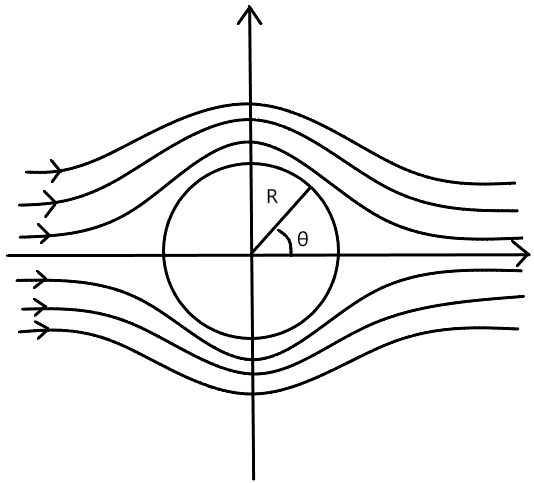
\includegraphics[width=70mm]{img/ryuutai1.png}
  \caption{円柱周りの流線}
\end{figure}
\par
このとき円柱周りの流体を理想流体とすると、揚力$L$は、円柱上の圧力$p$、円柱から十分に離れた場所での圧力$p_\infty$、円柱の半径$R$とすると、
\begin{align}
  L = -\int_0^{2\pi}(p-p_\infty)\sin\theta Rd\theta
\end{align}
ここで流速$U$、円柱上の速度$V$とすると、ベルヌーイの定理を用いて次のように表される。
\begin{align}
  \frac{p_\infty}{\rho} + \frac{U^2}{2} = \frac{p}{\rho} + \frac{V^2}{2}
\end{align}
これを変形すると
\begin{align}
  p-p_\infty = \frac{\rho(U^2-V^2)}{2}
  \label{eq:9}
\end{align}
この$V$を円柱が回転する場合と回転しない場合との複素ポテンシャルからそれぞれ求めていく。

\subsection{一様流と二重吹き出しの複素ポテンシャル}
回転しない円柱周りの複素ポテンシャルは、一様流と二重吹き出しの複素ポテンシャルの重ね合わせで表される。
一様流は場所によらず速度ベクトルが一定の流れであり、以下のような図で表される。
\begin{figure}[ht]
  \centering
  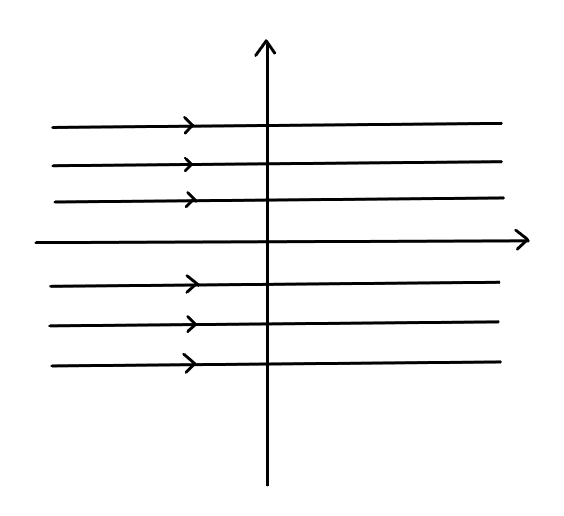
\includegraphics[width=60mm]{img/ryuutai3.png}
  \caption{一様流の例}
\end{figure}
\par
二次元流れにおいて$x$軸と角度$\alpha$をなす一様流の複素ポテンシャルは以下の形で表される。
\begin{align}
  W(z) = Ue^{-i\alpha}z
\end{align}
原点を円柱の中心とする二次元ポテンシャルにおいて$x$軸と平行な方向に流れる流体を考えた場合、$W(z) = Uz$である。
二重吹き出しは、流線が$y$軸上に中心を持ち、原点を通る円群で表される流れであり、図\ref{fig:3}のように表される。
\begin{figure}[ht]
  \centering
  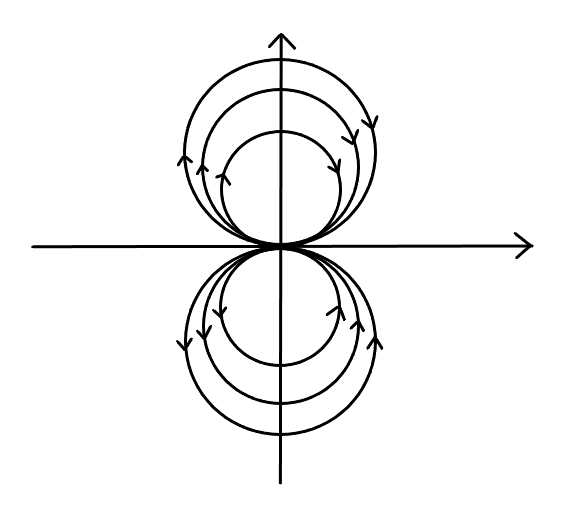
\includegraphics[width=60mm]{img/ryuutai2.png}
  \caption{二重吹き出しの例}
  \label{fig:3}
\end{figure}
今回の場合では$W(z) = \frac{R^2U}{z}$と表すことができる。これらを重ね合わせ、
\begin{align}
  W(z) = Uz + \frac{R^2U}{z}
\end{align}
で表される。ここで、$z = re^{i\theta}$を用いると
\begin{align}
  \frac{dW(z)}{dz}
  &= U - \frac{R^2U}{z^2}
  = U - \frac{R^2U}{r^2}e^{-2i\theta} \notag \\
  &= U - \frac{R^2u}{r^2}(\cos2\theta - i\sin2\theta)
  = u - iv
\end{align}
よって
\begin{align}
  u = U - \frac{R^2U}{r^2} \cos2\theta,\quad
  v = -\frac{R^2U}{r^2} \sin2\theta
\end{align}
円柱上では$r = R$であるから
\begin{align}
  V = \sqrt{u^2+v^2}
    = 2U|\sin\theta|
\end{align}
この$V$を(\ref{eq:9})式に代入し、$L$を求めると
\begin{align}
  p - p_\infty = \frac{\rho U^2(1 - 4\sin^2\theta)}{2}
\end{align}
\begin{align}
  L = -\frac{\rho U^2R}{2} \int_0^{2\pi} (1 - 4\sin^2\theta) \sin\theta d\theta 
    = 0
\end{align}
従って、一様流中の回転しない円柱には揚力は働かない事がわかる。
次に、円柱が回転している場合について考える。このとき複素ポテンシャルは一様流と二重吹き出しに加え、回転の強さを表す循環$\Gamma$を用いて次のように表される。
\begin{align}
  W(z) = Uz + \frac{UR^2}{z} + \frac{i\Gamma}{2\pi} \log z
\end{align}
ここで$z=re^{i\theta}$を使って、
\begin{align}
  \frac{dW(z)}{dz}
  = u - iv
  &= U - \frac{UR^2}{z^2} + i\frac{\Gamma}{2\pi z}
  = U - \frac{UR^2}{r^2}e^{-2i\theta} + i\frac{\Gamma}{2\pi z}e^{-i\theta}
\end{align}
よって
\begin{align}
  u &= U - \frac{UR^2}{r^2}\cos 2\theta + \frac{\Gamma}{2\pi r}\sin\theta,\\
  v &= -\frac{UR^2}{r^2}\sin 2\theta - \frac{\Gamma}{2\pi r}\cos\theta
\end{align}
円柱上では$r = R$であるからこれを代入すると、
\begin{align}
  u &= U(1 - \cos 2\theta) + \frac{\Gamma}{2\pi R}
    = (2U\sin\theta + \frac{\Gamma}{2\pi R})\sin\theta,\\
  v &= -U\sin\theta - \frac{\Gamma}{2\pi R}\cos\theta
    = -(2U\sin\theta + \frac{\Gamma}{2\pi R})\cos\theta,\\
  V &= \sqrt{u^2 + v^2} = \qty|2U\sin\theta + \frac{\Gamma}{2\pi R}|
\end{align}
これを(\ref{eq:9})式に代入し、$L$を求めると、
\begin{align}
  p - p_\infty &= \frac{\rho U^2}{2} \qty[1 - 4\qty(\sin\theta + \frac{\Gamma}{4\pi RU})^2],\\
  L &= -\frac{\rho U^2R}{2}\int_0^{2\pi} \qty[1 - 4\qty(\sin\theta + \frac{\Gamma}{4\pi RU})^2]\sin\theta d\theta %\\
    = \rho U\Gamma
  \label{eq:26}
\end{align}
従って、回転する円柱に働く揚力は、流体の密度、流速、循環の積で表すことができる。

\subsection{循環}
先程使った循環だが、一体どんな値であるかを具体的に説明する。
循環$\Gamma$は、流体中に閉曲線$C$をとり、$s$を閉曲線$C$に沿った長さ、$V$を閉曲線上の任意の点$P$における速度、$\theta$を$V$と点$P$での閉曲線の接線とのなす角とすると、次のように定義される。
\begin{align}
  \Gamma = \oint_C V\cos\theta ds
\end{align}
円柱の場合、半径$R$、周方向速度$V_\theta$とすると、
\begin{align}
  \Gamma = 2\pi RV_\theta
\end{align}
となる。この円柱が毎秒$n$回転しているとき、$V_\theta = 2\pi Rn$と求められる。
また、(\ref{eq:26})式でも求めた通り、循環がある一様流から物体は揚力を受けるが、これをクッタ―ジューコフスキーの定理という。
球技においても、ボールを回転させ、循環が生じることにより変化が生まれる。

\section{翼に働く揚力}
揚力を利用しているものとして代表的なのは飛行機だろう。
飛行機の翼は一見薄い翼にエンジンが付いているだけのように見えるが、実際には揚力を最大限受けられるような構造をしている。
ここからは流体の粘性についても考慮しつつ飛行機の翼の構造について解説する。
\par
飛行機の翼は以下のような構造をしており、大きな特徴として、流線型をしている、反りがある、迎え角がある、の3つが挙げられ、それぞれに意味が有る。
「反り」とはその名の通り翼の湾曲であり、背面は膨らんで、腹面はへこんだ形状をしている。
迎え角とは翼の前縁と後縁とを結んだ直線と流れの方向とのなす角である。
\vspace{2zw} %% 調整
\begin{figure}[ht]
  \centering
  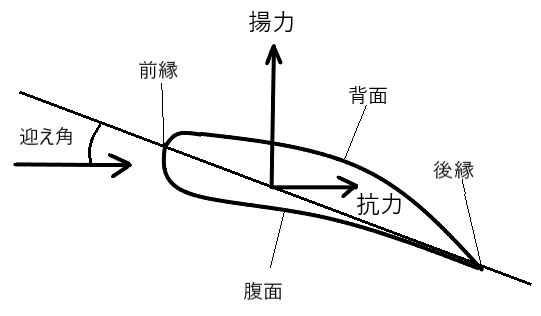
\includegraphics[width=70mm]{img/ryuutai4.png}
  \caption{翼の模式図}
\end{figure}

\subsection{流線形}
粘性のある流体では、物体のある一点から流線がはがれ、渦が発生する。
この流線がはがれる現象を剥離といい、はがれ始める点を剥離点という。
物体の後方で渦が発生し、流線が乱れると、前方と後方で圧力により作用する力に差が生じ、抗力が生じる。
この抗力を圧力抗力\footnote{抗力にはもう一つ摩擦抗力という物体表面に働く粘性摩擦による抗力があるが、圧力抗力に比べて非常に小さいので省略する。}といい、円柱のような流線形でない物体に比べて、流線形な物体は剥離点が後方にあるため、圧力抗力は低下する。
飛行機が流線形なのは流れと同じ方向(物体の進行方向とは逆方向)に働く圧力抗力を低下させるためである。
\begin{figure}[ht]
  \captionsetup{margin=0zw} % subcaption.sty
  \centering
  \begin{minipage}{0.49\textwidth}
    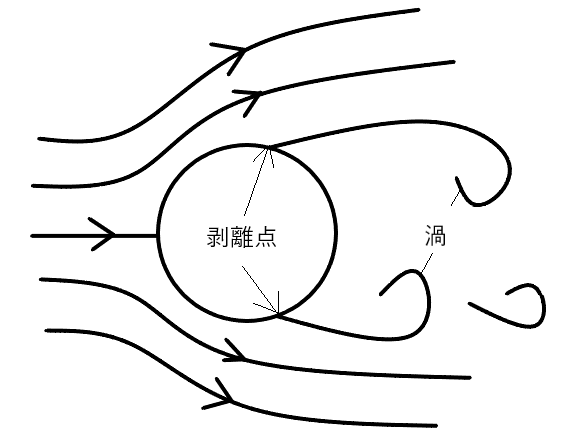
\includegraphics[width=\textwidth]{img/ryuutai5.png}
    \caption{円柱の剥離}
  \end{minipage}
  %
  \begin{minipage}{0.49\textwidth}
    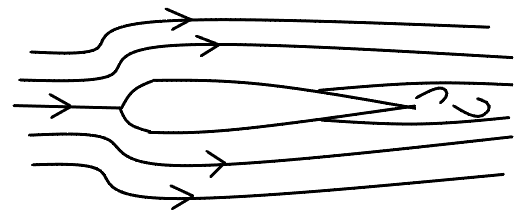
\includegraphics[width=\textwidth]{img/ryuutai6.png}
    \caption{流線形の物体の剥離}
  \end{minipage}
\end{figure}

\subsection{反り}
流体には曲面に沿って流れるという性質\footnote{コアンダ効果}があり、飛行機の翼にも関係する。
翼の上面に流れてきた流体は、翼の曲面に沿ってやや下向きに流れの方向を変える。
下面でも同様に、流体の流れはやや下に曲げられる。
要するに、翼の上面では翼が流体を下向きに引っ張り、下面では翼は流体を下向きに押している、という風に捉えることができる。
このとき、翼は作用反作用の原理で空気を下に引き付ける代わりに自身を上に引き上げている。
この引き上げる力が揚力であり、飛行機にとって欠かせない力となる。
\vspace{2zw} %% 調整
\begin{figure}[ht]
  \centering
  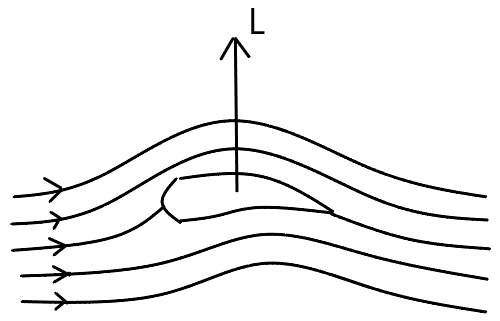
\includegraphics[width=70mm]{img/ryuutai7.png}
  \caption{翼まわりの流れ}
  \label{fig:7}
\end{figure}

\subsection{迎え角}
迎え角はレイノルズ数\footnote{補足にて解説}とともに揚力係数の値に関わっている。
揚力は、揚力係数$C_L$、流体の密度$\rho $、流速$U$、翼の面積$S$とすると次の式で表される。
\begin{align}
  L = \frac{1}{2}C_L\rho U^2S
\end{align}
一般的に揚力係数が大きいほど揚力は大きくなる。
レイノルズ数を一定にした場合の迎え角と揚力係数の変化は翼の特性曲線という曲線で表される。
\par
\begin{figure}[ht]
  \centering
  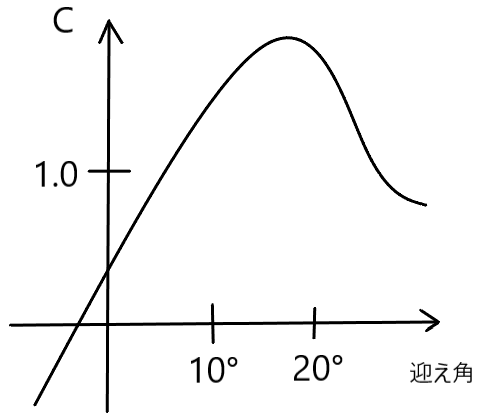
\includegraphics[width=60mm]{img/ryuutai8.png}
  \caption{翼の特性曲線}
\end{figure}
この図から、揚力係数は迎え角に比例するように増加し、ある一点で最大になり、その後は減少していくことがわかる。
これは迎え角が大きくなりすぎると剥離してしまうためであり、この現象を失速といい、揚力係数が最大になる迎え角を失速角という。
なお、翼の形状によって翼の特性曲線は異なり、上の図はあくまで一例に過ぎないが、揚力係数が迎え角の増加とともに直線的に増加していき、失速角で最大になった後急激に減少するという性質は共通している。

\section{翼の循環}
翼も円柱と同様に$L = \rho U\Gamma $が成り立つことがわかっている。
しかし、翼は円柱と違い回転が容易ではない。
それでは翼の何処に循環が存在するのか、ここでは二つの場合に分けて解説する。

\subsection{静止状態から動き始める場合}
翼が静止状態から動き出したとき、動き始めた瞬間は粘性の作用が遅れ、理想流体の流れが実現する。
このとき、前縁と後縁によどみ点\footnote{速度が$0$になる点}ができる。
すると後縁部では下から上へ回り込もうとするが、実在流体は粘性のために後縁を回って遡ることができず、よどみ点はより後方の先端へ移動する。
従って後縁部から流れ出て、図のように反時計回りに回転する渦ができる。
よって、翼の後方には後縁から離れた渦が残る。
翼が静止しているとき循環は$0$であり、渦は急に発生したり消滅したりしないので、反時計回りの渦を打ち消すために、時計回りの循環が翼まわりにできる。
こうして翼は循環流を得る。
\begin{figure}[ht]
  \centering
  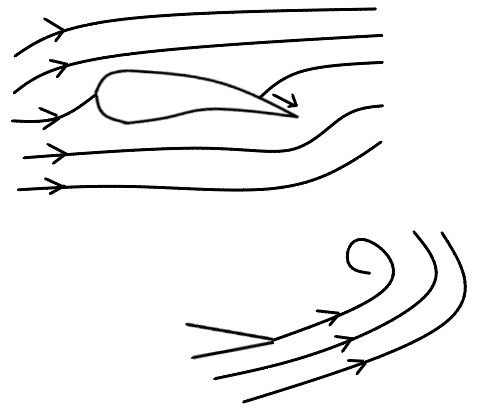
\includegraphics[width=60mm]{img/ryuutai9.png}
  \caption{理想流体としての流れと後縁にできる渦}
\end{figure}
\subsection{定常状態の場合}
図\ref{fig:7}に示された定常状態の流れは、流体が物体のまわりをまっすぐ流れていく一様流のような回転しない流れ\footnote{渦なし流れともいう}と流体が物体のまわりを回転している流れ\footnote{渦流れともいう}の重ね合わせたものになる。
後者の循環が$\Gamma $であるとき、翼の揚力は$\rho U\Gamma$となる。
\par
従って、翼が静止流体中を進行すると、翼まわりに循環が起こり、揚力が生じる。

\section{補足}
迎え角のところで少しだけ触れたが、レイノルズ数についてここで解説しておく。
レイノルズ数とは慣性力と粘性力の比であり、粘性の影響力を支配する無次元量である。
レイノルズ数$Re$は、代表速度$U$、代表長さ$L$、動粘度$\nu $とすると、次の式で表される。
\begin{align}
  Re = \frac{UL}{\nu}
\end{align}
レイノルズ数が非常に低ければ、粘性力が慣性力に比べて非常に大きいので、慣性力を無視することができる。
レイノルズ数が非常に高ければ、慣性力が支配する流れになり、粘性の影響は僅かになる。
レイノルズ数の値によって流れは大きく変化する。
レイノルズ数が$2300$以下では乱れのない直線及び曲線の流れであるのに対し、$2300$より大きいと不規則に乱れた流れになる。
このレイノルズ数を臨界レイノルズ数といい、乱れのない流れを層流、乱れた流れを乱流という。
\par
円柱周りの流れとレイノルズ数との関係を図に表した。
$0<Re<5$のとき、流線は対称になる。
$5\le Re<40$のとき、円柱の後方で剥離が起こり、双子渦と呼ばれる上下対称な渦ができる。
$40\le Re<150$のとき、定常流れであった流線が波打ち始め、円柱後方の上下2点から渦が交互に周期的に放出され、カルマン渦列という2本の渦列が形成される。
$150\le Re<300000$のとき、流れは円柱表面で剥離し、渦列は乱流に遷移し発達する。
$300000\le Re<3500000$のとき、円柱表面の流れも層流から乱流になり、渦の形成は弱くなる。
$3500000\le Re$のとき、 円柱表面で乱流となり、剥離点は後方に移動する。
\begin{figure}[ht]
  \centering
  \begin{minipage}{0.4\textwidth}
    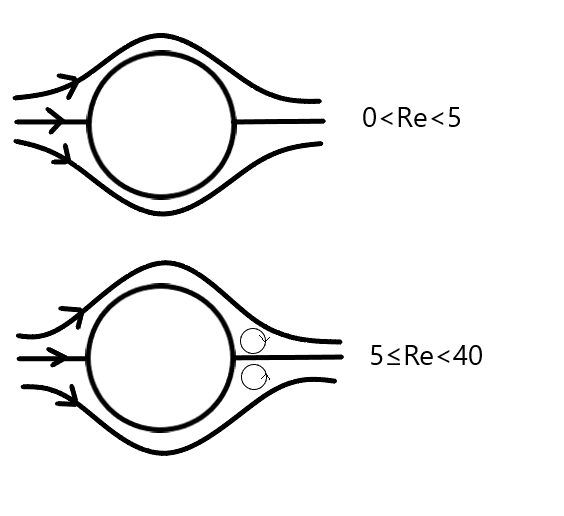
\includegraphics[width=\textwidth]{img/ryuutai10.png}
  \end{minipage}
  \qquad % 図の間の余白
  \begin{minipage}{0.4\textwidth}
    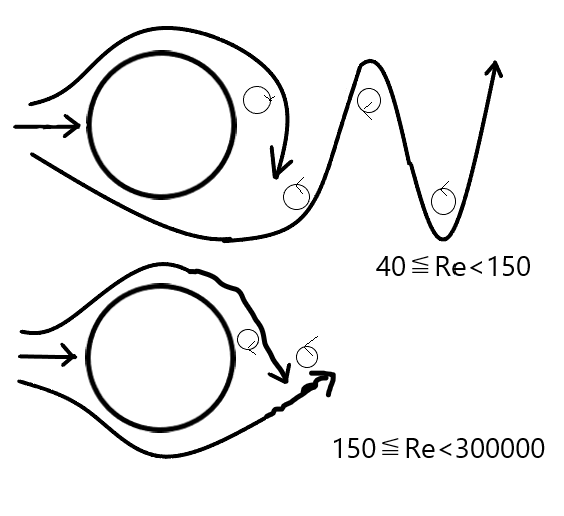
\includegraphics[width=\textwidth]{img/ryuutai11.png}
  \end{minipage}
  %
  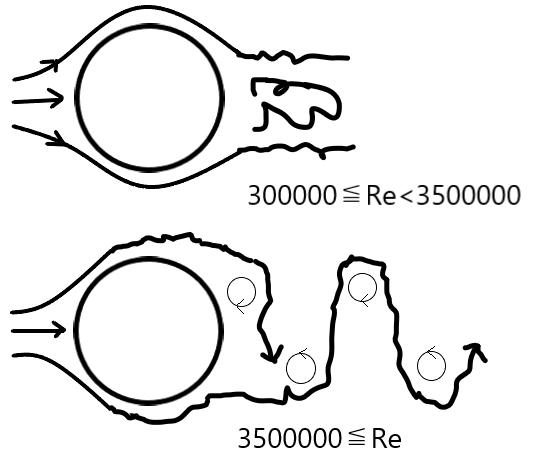
\includegraphics[width=0.4\textwidth]{img/ryuutai12.png}
  \caption{レイノルズ数と円柱まわりの流れ}
\end{figure}

\section{まとめ}
流体から揚力を得て利用しているのは人間に限ったことではない。
鳥の翼も迎え角、反りがある流線形のれっきとした翼である。
このように、揚力は人間だけでなく多くの生物にとって重要なものである。
ドローンやヘリコプターのローターも、実は飛行機の翼のような形状をしており、回転させることで揚力を得ることができる。
近い将来、人間が頭になんとかコプターをつけて空を飛べるようになるかもしれない。
流体は我々が常に触れ続けているが、とても複雑な運動をする物質でもある。
だが、複雑な流体を制御できて初めて我々は揚力を利用することができるのである。

% \clearpage
%% 参考文献
\begin{thebibliography}{99}
  \item 藤田勝久,『基本を学ぶ流体力学』,森北出版株式会社,2009.
  \item 石綿良三,『流体力学入門』,森北出版株式会社,2000.
  \item 石綿良三,『図解雑学流体力学』,ナツメ出版企画株式会社,2007.
\end{thebibliography}


\end{document}
%
% ファイトだよ!
%
